\documentclass[a4paper, 12pt]{article}
\usepackage{temp}
\usepackage{epsfig,graphicx,subfigure,amsthm,amsmath, float, xcolor, changepage, mathtools, textcomp, hyperref, bm, amssymb, tcolorbox, tikz, setspace}
\usepackage{array}
\usepackage[shortlabels]{enumitem}
\usepackage[bottom]{footmisc}
\usepackage{xepersian}
\settextfont[Scale=1]{XBZar}
%\setdigitfont{XBZar}
\setlatintextfont[Scale=0.9]{Times New Roman}
\hypersetup{
	colorlinks=true,
	urlcolor=blue!70!black
}

\newcolumntype{?}{!{\vrule width 1pt}}

\doublespacing
\begin{document}
\handout
{هوش مصنوعی}
{نیم‌سال اول
۱۴۰۱\lr{-}۱۴۰۰}
{دکتر محمدحسین رهبان}
{دانشکده مهندسی کامپیوتر}
{مینی‌پروژه چهارم - تئوری}
{محمدجواد هزاره}
{98101074}
\noindent
\\[-6em]
\section*{سوال ۱}
\begin{enumerate}[A)]
	\item
	ویژگی‌ها را شدت نور هر پیکسل در نظر می‌گیریم. بنابراین ورودی عکسی با $3\times 3$ پیکسل خواهد بود که 
	$x_{ij}$
	یک است، اگر پیکسل سطر $i$ و ستون $j$ روشن باشد و در غیر این‌صورت صفر خواهد بود. بنابراین با این تعاریف و با استفاده از \lr{Naive Bayes}، احتمال کلاس‌ها به صورت زیر خواهد بود:
	\[
	\prob\{C=A\} = \frac{1}{2},\qquad \prob\{C=B\} = \frac{1}{2}
	\]
	احتمال ویژگی‌ها به شرط کلاس‌ها نیز به صورت زیر خواهد بود که سطر $ij$ هر ماتریس، احتمال $x_{ij} = 1$ به شرط کلاس مورد نظر است:
	\[
	\prob\{X=1|C=A\} = \left(\begin{array}{ccc}
		\frac{1}{3} & \frac{2}{3} & \frac{1}{3} \\
		0 & 1 & 1 \\
		\frac{1}{3} & 0 & 0
	\end{array}\right), \qquad
	\prob\{X=1|C=B\} = \left(\begin{array}{ccc}
		\frac{1}{3} & \frac{1}{3} & \frac{2}{3} \\
		\frac{2}{3} & \frac{1}{3} & 0\\
		\frac{2}{3} & 1 & 0
	\end{array}\right)
	\]
	با توجه به صفر شدن احتمال‌ها استفاده از روش \lr{Laplace smoothing} ر در نظر می‌گیریم. ضریب \lr{smoothing} را برابر $2$ در نظر گرفته و درنتیجه احتمال‌ها به صورت زیر آپدیت خواهند شد:
	\[
	\prob\{X=1|C=A\} = \left(\begin{array}{ccc}
		\frac{3}{7} & \frac{4}{7} & \frac{3}{7} \\
		\frac{2}{7} & \frac{5}{7} & \frac{5}{7} \\
		\frac{3}{7} & \frac{2}{7} & \frac{2}{7}
	\end{array}\right), \qquad
	\prob\{X=1|C=B\} = \left(\begin{array}{ccc}
		\frac{3}{7} & \frac{3}{7} & \frac{4}{7} \\
		\frac{4}{7} & \frac{3}{7} & \frac{2}{7}\\
		\frac{4}{7} & \frac{5}{7} & \frac{2}{7}
	\end{array}\right)
	\]
	بنابراین برای داده‌ی ورودی می‌توان احتمال تعلق آن به هر کلاس را محاسبه کرد:
	\[
	\begin{aligned}
		&\prob\{C=A|X_{new}\} = \prob\{C=A\}\prob\{X_{new}|C=A\} = \frac{1}{2} \times \frac{4}{7} \times \frac{4}{7} \times \frac{4}{7} \times \frac{5}{7} \times \frac{5}{7} \times \frac{5}{7} \times \frac{3}{7} \times \frac{2}{7} \times \frac{5}{7} = \frac{240,000}{2\times 7^9}\\[0.4em]
		&\prob\{C=A|X_{new}\} = \prob\{C=A\}\prob\{X_{new}|C=A\} = \frac{1}{2} \times \frac{4}{7} \times \frac{3}{7} \times \frac{3}{7} \times \frac{3}{7} \times \frac{3}{7} \times \frac{2}{7} \times \frac{4}{7} \times \frac{5}{7} \times \frac{5}{7} = \frac{64,800}{2\times 7^9}
	\end{aligned}
	\]
	بنابراین با توجه به این‌که
	$\prob\{C=A|X_{new}\} > \prob\{C=B|X_{new}\}$،
	داده‌ی جدید به کلاس $A$ تعلق خواهد گرفت.
	\item
	کافیست درختی بسازیم که در هر راس آن براساس روشن یا خاموش بودن پیکسل‌ها بتوان به بچه‌ی راست و چپ آن راس رفت و هر یک از برگ‌ها نیز برچسب یکی از کلاس‌های مسئله را خواهند داشت. با داشتن این درخت، برای یک داده‌ی جدید کافیست براساس روشن و یا خاموش بودن پیکسل‌های آن بر روی درخت حرکت کنیم تا به یک برگ برسیم و برچسب این برگ را به عنوان کلاس این داده خروجی دهیم.
\end{enumerate}

\pagebreak
\section*{سوال ۲}
فرض کنیم داده‌ی ورودی به صورت
$\mathcal{D} = \{x_i, y_i\}_{i=1}^{i=m}$
باشد. تعاریف زیر را در نظر می‌گیریم:
\[
\begin{dcases}
	B = \min A, \quad A = \{\|w\|_2 \,|\, \forall i \in [m]: y_i \langle w, x_i \rangle \ge 1\} \\
	R = \max_i \|x_i\|_2
\end{dcases}
\]
هم‌چنین فرض می‌کنیم الگوریتم با $w=0$ شروع می‌کند و در مرحله‌ی آپدیت، بردار وزن به صورت
$w^{t+1} = w^{t} + y_ix_i$
آپدیت می‌شود. (که فرض شده $\eta = 1$؛ برای $\eta \ne 1$ کافیست ورودی‌های مسئله را  \lr{scale} کنیم.) نشان می‌دهیم کران‌بالای دفعاتی که مراحل الگوریتم تکرار خواهند شد برابر با
$(RB)^2$
خواهد بود. برای این منظور، بردار $\bm{\hat{n}}$ را بردار یکه در راستای متناظر با $w$ای در نظر می‌گیریم که $B$ را بدست می‌آورد. به عبارتی خواهیم داشت:
\[
\forall i \in \{1, \cdots, m\}: y_i\langle B\bm{\hat{n}}, x_i\rangle \ge 1 \qquad (\ast)
\]
فرض کنیم الگوریتم $k$ بار اجرا می‌شود. هدف پیدا کردن کرانی برای $k$ است. حال اگر در مرحله‌ی $t$ام، داده‌ی $j$ام اشتباه دسته‌بندی شده باشد، آن‌گاه
$\bm{w^{t+1}} = \bm{w^{t}} + y_j\bm{x_j}$.
بنابراین داریم:
\[
\begin{aligned}
	\begin{aligned}
		\langle\bm{w^{t+1}}, B\bm{\hat{n}}\rangle &= B \langle\bm{w^t + y_j\bm{x_j}}, \bm{\hat{n}}\rangle \\
		&= B \left(\langle\bm{w^t}, \bm{\hat{n}}\rangle + \langle y_j\bm{x_j}, \bm{\hat{n}}\rangle\right)
	\end{aligned} \\[1.5em]
	\begin{aligned}
		\implies\langle\bm{w^{t+1}}, \bm{\hat{n}} \rangle &= \langle\bm{w^t}, \bm{\hat{n}}\rangle + \frac{1}{B} \langle y_j\bm{x_j}, B\bm{\hat{n}}\rangle \\
		&\ge \langle\bm{w^t}, \bm{\hat{n}}\rangle + \frac{1}{B}
	\end{aligned}
\end{aligned}
\]
که خط آخر با توجه به $(\ast)$ نتیجه شده است. حال با توجه به استقرا و این‌که 
$\bm{w^1} = \bm{0}$
، برای هر $t$ در بازه‌ی ۱ تا $k$ خواهیم داشت: (تمامی نرم‌ها $L_2$ هستند.)
\[
\langle\bm{w^{t+1}}, \bm{\hat{n}}\rangle \ge \frac{t}{B} \xRightarrow{\|\bm{\hat{n}}\| = 1} \|\bm{w^{t+1}}\| \ge \frac{t}{B} \qquad (\star)
\]
هم‌چنین برای
$\|\bm{w^{t+1}}\|$
داریم:
\[
\begin{aligned}
	\|\bm{w^{t+1}}\|^2 &= \|\bm{w^t} + y_j\bm{x_j}\|^2 \\
	&= \|\bm{w^t}\|^2 + y_j^2\|\bm{x_j}\|^2 + 2\langle\bm{w^t}, y_j\bm{x_j}\rangle \quad (\diamond)
\end{aligned}
\]
و از آن‌جایی که فرض کرده بودیم داده‌ی $j$ام اشتباه دسته‌بندی شده است،
$\langle\bm{w^{t}}, y_j\bm{x_j}\rangle \le 0$
خواهد بود و هم‌چنین مطابق تعریف الگوریتم برچسب‌ها یک یا منفی یک بودند که نتیجه می‌دهد $y_j^2 = 1$. مطابق تعریف $R$ برای هر $i$، خواهیم داشت
$\|\bm{x_i}\| \le R$
؛ با توجه به این موارد داریم:
\[
\begin{aligned}
	(\diamond) \implies \|\bm{w^{t+1}}\|^2 \le \|\bm{w^t}\|^2 + R^2 
\end{aligned}
\]
با استفاده از استقرا خواهیم داشت:
\[
\|\bm{w^{t+1}}\|^2 \le t\,R^2 \qquad (\star\star)
\]
با کنار هم گذاشتن
$(\star)$
و
$(\star\star)$
و قرار دادن $k$ به جای $t$ خواهیم داشت:
\[
\frac{k^2}{B^2} \le \|\bm{w^{t+1}}\|^2 \le k\,R^2 \implies \boxed{k \le B^2R^2}
\]
بنابراین حداکثر دفعات تکرار مراحل الگوریتم برابر $B^2R^2$ خواهد بود.

\pagebreak
\section*{سوال ۳}
نخست شبکه‌ای که تسخیص دهد ورودی در هر یک از نواحی شماره‌گذاری شده‌ی تصویر زیر باشد را ساخته و سپس با ااجتماع گرفتن بین این شبکه‌ها، خواسته‌ی اصلی مسئله برآورده می‌شود.
\begin{figure}[H]
	\centering
	\includegraphics[width=0.5\textwidth]{3.png}
\end{figure}
\noindent
برای هر یک از نواحی نیز، باید تشخیص دهیم ورودی سمت چپ مرزهای آن ناحیه باشد. برای تابع \lr{activation} نیز از تابع $f$ استفاده می‌کنیم که به صورت زیر تعریف می‌شود:
\[
f(x) = \begin{dcases}
	1 &\quad x > 0\\
	0 &\quad x \le 0
\end{dcases}
\]
بنابراین:
\begin{figure}[H]
	\centering
	\includegraphics[width=0.45\textwidth]{3-2.png}
	\hspace*{0.05\textwidth}
	\includegraphics[width=0.45\textwidth]{3-4.png}
\end{figure}
\begin{figure}[H]
	\centering
	\includegraphics[width=0.45\textwidth]{3-3.png}
	\hspace*{0.05\textwidth}
	\includegraphics[width=0.45\textwidth]{3-1.png}
\end{figure}
\noindent
کافیست خروجی‌های $y_1$ تا $y_4$ را با یکدیگر \lr{or} کنیم. بنابراین:
\begin{center}
	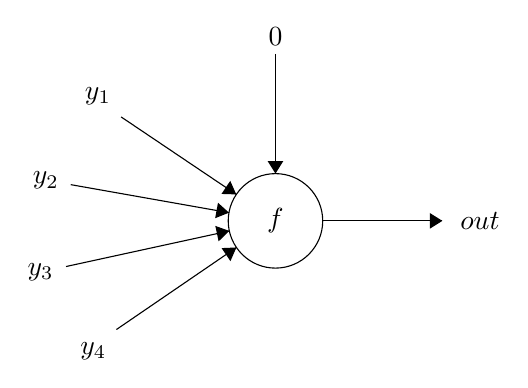
\begin{tikzpicture}[scale=0.2]
		\tikzstyle{every node}+=[inner sep=0pt]
		\draw [black] (39.4,-29.1) circle (3);
		\draw (39.4,-29.1) node {$f$};
		\draw [black] (29.6,-22.5) -- (36.91,-27.42);
		\draw (28.99,-21.16) node [left] {$y_1$};
		\fill [black] (36.91,-27.42) -- (36.53,-26.56) -- (35.97,-27.39);
		\draw [black] (26.4,-26.8) -- (36.45,-28.58);
		\draw (25.68,-26.55) node [left] {$y_2$};
		\fill [black] (36.45,-28.58) -- (35.75,-27.95) -- (35.57,-28.93);
		\draw [black] (26.1,-32) -- (36.47,-29.74);
		\draw (25.35,-32.36) node [left] {$y_3$};
		\fill [black] (36.47,-29.74) -- (35.58,-29.42) -- (35.79,-30.4);
		\draw [black] (29.3,-36) -- (36.92,-30.79);
		\draw (28.7,-37.35) node [left] {$y_4$};
		\fill [black] (36.92,-30.79) -- (35.98,-30.83) -- (36.54,-31.66);
		\draw [black] (50,-29.1) -- (42.4,-29.1);
		\draw (51.1,-29.1) node [right] {$out$};
		\fill [black] (50,-29.1) -- (49.2,-29.6) -- (49.2,-28.6);
		\draw [black] (39.4,-18.5) -- (39.4,-26.1);
		\draw (39.4,-18) node [above] {$0$};
		\fill [black] (39.4,-26.1) -- (39.9,-25.3) -- (38.9,-25.3);
	\end{tikzpicture}
\end{center}
که وزن یال‌های متصل‌کننده‌ی $y_i$ها به این نورون همگی برابر $1$ است.
\end{document}



